%%%%%%%%%%%%%%%%%%%%%%%%%%%%%%%%%%%%%%%%%
%
% Funkcionalna verifikacija hardvera
% 
%%%%%%%%%%%%%%%%%%%%%%%%%%%%%%%%%%%%%%%%%

Ova i naredne vežbe su posvećene univerzalnoj verifikacionoj metodologiji.
U ovoj vežbi je dat kratak pregled metodologije i objašnjeni osnovni koncepti.
Data je funkcionalna specifikacija dizajna koji će se verifikovati i opis
transakcija.
Naredne vežbe su posvećene pojedinim komponentama, njihovoj ulozi i načinu
korišćenja.

%========================================================================================
% Section
%========================================================================================

\section{Uvod}

UVM (engl. \emph{Universal Verification Methodology}) je standardizovana
metodologija za funkcionalnu verifikaciju sa pomoćnom bibiliotekom u
SystemVerilog jeziku. Kreirala ju je firma Accellera u saradnji sa mnogim EDA
prodavcima i klijentima sa željom da se postigne lakša ponovna upotreba
testbenčeva i jednostavno kreiranje univerzalnih, visoko-kvalitetnih VIP-a
(engl. \emph{Verification Intellectual Property}). UVM je baziran na OVM-u
(engl. \emph{Open Verification Methodology}) i eRM-u (engl. \emph{e Resuse
  Methodology}).\\

Jedna od glavnih karakteristika ove metodologije je UVC (engl. \emph{Universal
  Verification Component}), odnosno univerzalne verifikacione komponente koje
imaju istu strukturu (sadrže monitore, drajvere, sekvencere, ...) što omogućava
lako korišćenje bilo kako nezavisne komponente ili kao deo većeg sistema.\\

Objektno-orijentisani dizajn, kao glavna karakteristika SystemVerilog jezika,
omogućava lako kreiranje verifikacionih komponenti, dok veliki broj
predefinisanih funkcija i taskova znatno ubrzava proces kreiranja testova.\\

UVM obezbeđuje \emph{framework} za verifikaciju zasnovanu na pokrivenosti
(engl. \emph{Coverage Driven Verification}, skraćeno CDV) koja ne zahteva
kreiranje velikog broja testova, osigurava temeljnu verifikaciju na osnovu
zadatih parametara i olakšava proces pronalaženja problema. Ovo se postiže
korišćenjem \emph{self-checking} testbenčeva, automatskog generisanja testova i
korišćenjem podataka o pokrivenosti.

% ----------------------------------------------------------------------------------------

\subsection{Istorijat}

UVM 1.0 je nastao 2011 godine i, zbog velike podrške simulatora, ubrzo zamenio,
do tada popularni, OVM. UVM 1.0 je preuzeo dosta iz OVM 2.1.1 verzije (u velikom
delu koda samo zamenjujući prefikse ``ovm\(\_\)'' sa ``uvm\(\_\)'') i dodao par
nadogradnji koje umnogome olakšavaju upotrebu i pružaju veću funkcionalnost.
Među njima su \emph{end-of-test} mehanizam za olakšavanje završavanja testova,
\emph{callback} mehanizam, lakša podešavanja izveštaja, ... UVM 1.0 je pratilo
nekoliko manjih izdanja gde su ispravljene sitne greške i dodate nove
funkcionalnosti uključujući registarski sloj, faze, sekvence, TLM interfejse,
... Trenutna verzija UVM-a je UVM 1.2 koji je izašao 2014 godine. UVM
biblioteka, kao i prethodne verzije se mogu preuzeti sa
\url{http://www.accellera.org/downloads/standards/uvm}

%========================================================================================
% Section
%========================================================================================

\section{UVM verifikaciono okruženje}

U ovom poglavlju je dat kratak pregled klasičnog UVM testbenča. Ukratko je
objašnjena struktura testbenča, navedene osnovne komponente, način kreiranja
testova, ali i osnovni elementi UVM biblioteke. Dat je samo kratak pregled i
uloga, a sve komponente i navedene UVM-ove mogućnosti će biti detaljno
razrađene u narednim vežbama.

% ----------------------------------------------------------------------------------------

\subsection{Tipična struktura testbenča}

Svaki UVM testbenč se sastoji od određenog broja verifikacionih komponenti sa
jasno definisanom ulogom, koje su povezane na odgovarajući način, prate
metodologiju i omogućavaju laku ponovnu upotrebu. Na blok dijagramu (slika
\ref{fig:typical_tb}) je prikazana tipična struktura testbenča.\\

\begin{figure}[h!]
  \centering
  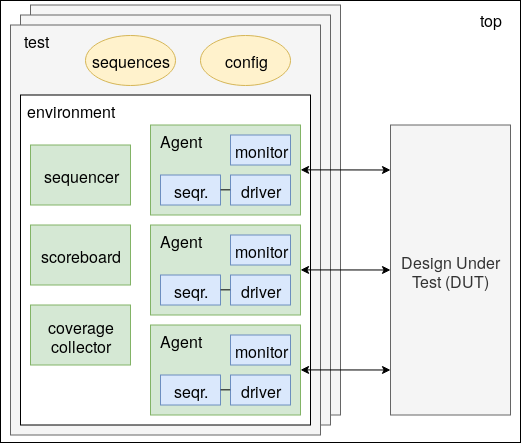
\includegraphics[width=100mm]{img/v5_typical_tb.png}
  \caption{UVM testbenc}
  \label{fig:typical_tb}
\end{figure}

Prikazani delovi testbenča su:
\begin{itemize}
\item \emph{data objekat} (paket, \emph{sequence item}, transaction) - koristi
  se kao stimulus za dizajn koji se verifikuje. Mora sadržati polja koja su
  potrebna drajveru da bi uspešno inicirao transakciju, ali može sadržati i neka
  dodatna polja koja se koriste za kontrolu, kao i ograničenja pri randomizaciji
\item sekvencer komponenta - je stimulus generator. U njemu se kontrolišu podaci
  koje će drajver slati DUT-u. Kontrola podataka se vrši u definisanim
  sekvencama koje određuju broj paketa, redosled, sadržaj i sl. Kreiranje
  sekvenci je glavni način generisanja stimulusa u UVM-u
\item drajver komponenta - je aktivna komponenta koja emulira signale koji se
  šalju dizajnu. Na osnovu podataka od sekvencera i semplovanja signal na
  interfejsu, generiše signale na ulaze dizajna koji se verifikuje, prateći
  implementirani protokol
\item monitor komponenta - je pasivna komponenta zadužena za nadgledanje
  signala, ali ne i njihovo generisanje. Može sakupljati podatke o pokrivenosti,
  ali i raditi proveru. Sakupljene informacije šalje ostalim komponentama na
  dalju obradu (npr. \emph{scoreboard}-u na dalju kontrolu)
\item agent komponenta - obuhvata drajver, sekvencer i monitor. Iako se ove
  podkomponente mogu koristiti nezavisno to iziskuje poznavanje imena, uloge i
  načina povezivanja. Agent obuhvata ove tri komponente, predstavlja
  apstraktniji pristup datom interfejsu i olakšava ponovno korišćenje ovih
  komponenti. Aktivan agent instancira sve tri komponente, dok pasivan
  instancira samo monitor (pasivan agent ne generiše signale, služi samo za
  nadgledanje; uglavnom je deo većeg okruženja, gde se generisanje podataka vrši
  na nekom višem nivou)
\item \emph{scoreboard} - na osnovu podataka dobijenih iz monitora vrši proveru
\item konfiguracioni objekat - sadrži sve podatke potrebne za konfigurisanje
  testbenča npr. broj agenata, da li je potreban master ili \emph{slave}, da li
  je agent aktivan ili pasivan i sl.
\item okruženje - obuhvata sve prethodno navedene delove u jednu klasu radi
  jednostavnog korišćenja
\item test
\end{itemize}

Hijerarhija testbenča je određena nizom \emph{has-a} klasnim vezama tj.
komponente na višem nivou hijerarhije sadrže komponente na nižem nivou. Npr.
agent sadrži drajver, sekvencer i monitor. Ovo je prikazano na slici
\ref{fig:uvm_hierarchy}.\\

\begin{figure}[h!]
  \centering
  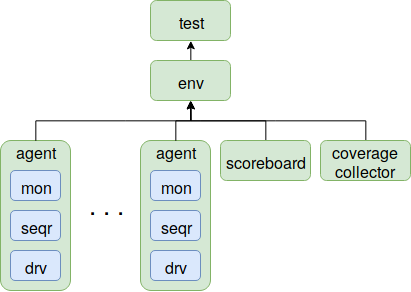
\includegraphics[width=80mm]{img/v5_uvm_hierarchy.png}
  \caption{UVM hijerarhija}
  \label{fig:uvm_hierarchy}
\end{figure}

Sa ove slike se vidi i da je test na najvišem nivou hijerarhije. On je zadužen
za instanciranje i konfiguraciju okruženja i startovanje sekvenci. Često postoji
bazna test klasa u kojoj se vrše instanciranje okruženja, dok se u izvedenim
testovima vrše specifične operacije za taj test npr. redosled sekvenci,
randomizacija i sl.

% ----------------------------------------------------------------------------------------

\subsection{UVM klasna hijerarhija}

Na slici \ref{fig:uvm_class_hierarchy} je prikazana delimična UVM klasna
hijerarhija.
Nasleđivanje omogućava brz razvoj dobro struktuiranih verifikacionih komponenti
i objekata. Bazne klase sadrže potrebna polja i metode za kontrolu, pa je,
umesto pisanja svake komponente od nule, potrebno samo modifikovati određene
metode za konkretne potrebe.\\

\begin{figure}[h!]
  \centering
  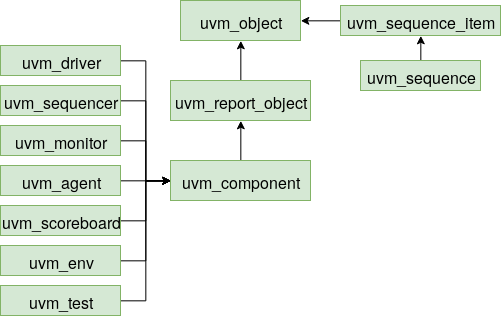
\includegraphics[width=100mm]{img/v5_uvm_class_hierarchy.png}
  \caption{UVM klasna hijerarhija}
  \label{fig:uvm_class_hierarchy}
\end{figure}

Kao što se vidi sa slike \ref{fig:uvm_class_hierarchy}, svaki deo testbenča
opisan u prethodnom poglavlju ima odgovarajuću UVM klasu i kako bi se
implementirao potrebno je naslediti tu klasu.
Npr. ukoliko želimo da implementiramo monitor, potrebno je napisati novu klasu
koja nasleđuje \emph{uvm\(\_\)monitor}.
Slično će drajver nasleđivati \emph{uvm\(\_\)driver}, sekvencer
\emph{uvm\(\_\)sequencer} i sl.\\

Takođe se može uočiti da sve klase nasleđuju \emph{uvm\(\_\)object} klasu.
Jedna od bitnijih podklasa je \emph{uvm\(\_\)component}. Klasa komponenta je
izvedena iz klase objekat, međutim sadrži veoma bitne osobine zbog kojih se
često posebno izdvaja. Prvenstveno sadrži UVM-ov mehanizam faza, mogućnost
korišćenja konfiguracija i TLM interfejse. Sve klase koje se koriste za
kreiranje komponenti verifikacionog okruženja (\emph{uvm\(\_\)driver},
\emph{uvm\(\_\)monitor}, \emph{uvm\(\_\)env}, ...) nasleđuju
\emph{uvm\(\_\)component} klasu. Obično se u literaturi kao dve glavne grupe
navode objekti i komponente, pri čemu se pravi razlika između klasa nasleđenih
iz \emph{uvm\(\_\)object} i klasa nasleđenih iz \emph{uvm\(\_\)component} (iako
su i ove klase naseđene iz \emph{uvm\(\_\)object}, izdvajaju se zbog velikog
broja posebnih osobina).

% ----------------------------------------------------------------------------------------

\subsection{UVM faze}

UVM-ov mehanizam faza je jedna od najbitnijih funkcionalnosti i novina u ovoj
biblioteci. Kao što je već navedeno, jedna od osnovnih mogućnosti
\emph{uvm\(\_\)component} klase su upravo faze. Pošto u verifikacionom okruženju
postoji veliki broj komponenti koje rade u paraleli, potrebno je obezbediti da
se određene funkcionalnosti izvrše u jasno definisanim trenucima. Faze
predstavljaju sinhronizacioni mehanizam za okruženje odnosno sve komponente su
uvek sinhronizovane u pogledu faza.\\

Postoje tri osnovne grupe UVM faza:
\begin{itemize}
\item \emph{build} faze - za kreiranje i konfigurisanje okruženja
\item \emph{run-time} faze - gde zapravo teče simulaciono vreme
\item \emph{clean up} faze - sakupljanje i analiza rezultata
\end{itemize}

Ove faze su zapravo samo virtuelne metode u \emph{uvm\(\_\)component} klasi,
čijim se modifikacijama omogućava jasno definisan \emph{flow} u okruženju.
Korišćenjem faza se povećava mogućnost ponovne upotrebe komponenti jer je uloga
svake faze, i funkcionalnosti koje se u njoj izvršavaju, jasno definisana. Na
slici \ref{fig:uvm_phases} su prikazane sve UVM faze i grupisane u tri osnovne
grupe.\\

\begin{figure}
  \centering
  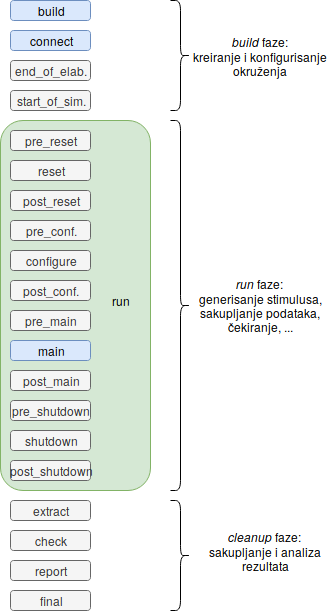
\includegraphics[width=80mm, scale=0.5]{img/v5_uvm_phases.png}
  \caption{UVM faze}
  \label{fig:uvm_phases}
\end{figure}

U tabeli \ref{tab:uvm_phases} je dat kratak opis svih faza u redosledu izvršavanja.\\

\begin{table}[h!]
  \centering
  \rowcolors{1}{white!15}{gray!30}
  \begin{tabular}{|p{0.2\textwidth}|p{0.7\textwidth}|}
    \hline
    \textbf{Faza} & \textbf{Opis} \\
    \hline
    \emph{build} & instanciranje podkomponenti, podešavanje konfiguracija, ...\\
    \hline
    \emph{connect} & međusobno povezivanje komponenti, podešavanje interfejsa, ...\\
    \hline
    \emph{end\(\_\)of\(\_\)elaboration} & prikaz topologije, naknadne izmene (u ovoj fazi je okruženje potpuno kreirano i povezano)\\
    \hline
    \emph{start\(\_\)of\(\_\)simulation} & prikaz topologije, priprema za početak simulacije, podešavanja \emph{run-time} konfiguracija, simulatora, ...\\
    \hline
    \emph{run} & sama simulacija (generisanje stimulusa, provera, ...)\\
    \hline
    \emph{extract} & preuzimanje preostalih podataka iz komponenti (npr. informacije iz \emph{scoreboard}-a ili monitora)\\
    \hline
    \emph{check} & preostale provere\\
    \hline
    \emph{report} & prikaz rezultata ili upis rezultata u fajlove\\
    \hline
    \emph{final} & završetak svih preostalih radnji (npr. zatvaranje fajlova ili terminacija simulatora)\\
    \hline
  \end{tabular}
  \caption{UVM faze}
  \label{tab:uvm_phases}
\end{table}

\emph{Run} faza ima veliki broj pod-faza koijma se može vršiti detaljnija
sinhronizacija. One su date u tabeli \ref{tab:uvm_run_phases}.\\

\begin{table}[h!]
  \centering
  \rowcolors{1}{white!15}{gray!30}
  \begin{tabular}{|p{0.2\textwidth}|p{0.7\textwidth}|}
    \hline
    \textbf{Faza} & \textbf{Opis} \\
    \hline
    \emph{pre\(\_\)reset} & sve aktivnosti koje treba obaviti pre reseta\\
    \hline
    \emph{reset} & specifično ponašanje tokom reseta\\
    \hline
    \emph{post\(\_\)reset} & sve aktivnosti koje treba obaviti nakon reseta\\
    \hline
    \emph{pre\(\_\)configure} & priprema DUT-a za konfiguraciju posle reseta\\
    \hline
    \emph{configure} & konfigurisanje DUT-a\\
    \hline
    \emph{post\(\_\)configure} & čekanje da DUT odreaguje na konfiguraciju\\
    \hline
    \emph{pre\(\_\)main} & provera da su sve komponente spremne za rad\\
    \hline
    \emph{main} & glavna faza - generisanje stimulusa, sakupljanje podataka, čekiranje, ...\\
    \hline
    \emph{post\(\_\)main} & finalizacija aktivnosti iz \emph{main} faze\\
    \hline
    \emph{pre\(\_\)shutdown} & pomoćna faza za aktivnosti pre \emph{shutdown} faze\\
    \hline
    \emph{shutdown} & provera da je generisan stimulus korektno propagiran, provera statusnih registara, ...\\
    \hline
    \emph{post\(\_\)shutdown} & finalizacija aktivnosti, poslednja aktivna faza\\
    \hline
  \end{tabular}
  \caption{UVM \emph{run} faze}
  \label{tab:uvm_run_phases}
\end{table}

UVM pruža velike mogućnosti pri korišćenju ovih faza.
Kao što se vidi, \emph{run-time} faze obuhvataju veliki broj pod-faza čija je
preporučena uloga i redosled jasno definisan.
Radi lakšeg prelaska sa OVM-a na UVM, omogućeno je korišćenje i samo \emph{run}
faze umesto svih pod-faza (pogledati sliku \ref{fig:uvm_phases}, \emph{run}
obuhvata \emph{reset}, \emph{main}, \emph{post\(\_\)main}, ..).\\

Dve najčešće korišćene faze su \emph{build} i \emph{run} (ili \emph{main}), pa
će kostur većine komponenti biti (primetiti da je \emph{run/main} faza
implementirana kao task zato što troši simulaciono vreme):

\begin{lstlisting}
class example extends uvm_component;

  // polja i podkomponente
  // ...

  `uvm_component_utils(example) // factory registration

  function new(string name = "example", uvm_component parent);
    super.new(name, parent);
  endfunction : new

  function void build_phase(uvm_phase phase);
    super.build_phase(phase);
    // ...
  endfunction : build_phase

  task main_phase(uvm_phase phase);
    super.main_phase(phase);
    // ...
  endtask : main_phase

endclass : example
\end{lstlisting}

% ----------------------------------------------------------------------------------------

\subsection{UVM \emph{factory}}

\emph{Factory} metoda je jedna od klasičnih softverskih dizajn šablona (engl.
\emph{desing pattern}). Prilikom funkcionalne verifikacije često je potrebno
uvesti promene u određenim klasama. Ovo se može desiti zbog uvođenja nove
funkcionalnosti, specifičnih zahteva nekog testa i sl. Na primer, možda je
potrebno dodati nova polja u transakciju ili modifikovati način generisanja
signala ili neka ograničenja pri randomizaciji. UVM \emph{factory} omogućava
jednostavan način zamene postojeće klase izvedenom klasom bez menjanja ostatka
okruženja. Primer: ukoliko u okruženju koristimo \emph{old\(\_\)transaction}
klasu za slanje podataka, a želimo da koristimo \emph{new\(\_\)transaction} koja
ima dodata određena ograničenja za randomizaciju potrebna za dati test. Ovo je
moguće postići jednom linijom koda. Tada se sve instance
\emph{old\(\_\)transaction} klase zamenjuju sa \emph{new\(\_\)transaction}, bez
menjanja ostatka koda. Odnosno u celom okruženju se koristi
\emph{new\(\_\)transaction} umesto \emph{old\(\_\)transaction}. Ovaj mehanizam
se naziva \emph{factory override} i biće obrađen u narednim vežbama.\\

Kako bi ovo bilo moguće, potrebno je pratiti određena pravila prilikom
implementacije klasa, objašnjena u nastavku. Konvencija je uvek pisati kod na
ovaj način radi lakše ponovne upotrebe.

\subsubsection{Registracija}

UVM objekti i komponente treba da sadrže kod za \emph{factory} registraciju koji
sadrži \emph{wrapper} klasu oko date klase (mora biti \emph{typedef}-ovana na
\emph{type\(\_\)id}), statičnu funkciju da se dobije ovaj \emph{type\(\_\)id}) i
funkciju za dobijanje imena tipa. Međutim, pošto se pri svakoj registraciji
moraju obaviti ovi koraci, koji prate dati šablon, razvijeni su određeni
\emph{factory registration} makroi. Konvencija je koristiti ove makroe umesto
ručnog pisanja potrebnog koda kako bi se izbegle eventualne greške i povećala
čitljivost koda. Postoje četiri makroa:

\begin{itemize}
\item \`\ uvm\(\_\)component\(\_\)utils(\textless name\textgreater ) - za komponente
\item \`\ uvm\(\_\)component\(\_\)param\(\_\)utils(\textless name\textgreater ) -
  za parametrizovane komponente
\item \`\ uvm\(\_\)object\(\_\)utils(\textless name\textgreater ) - za objekte
\item \`\ uvm\(\_\)object\(\_\)param\(\_\)utils(\textless name\textgreater ) - za
  parametrizovane objekte
\end{itemize}

Ukoliko je potrebno i korišćenje \emph{field} makroa, umesto ovih koriste se
\emph{begin..end} makroi koji kreiraju blok unutar kojeg se navode \emph{field}
makroi. Npr.

\begin{lstlisting}
`uvm_object_utils_begin(<tip>)
  `uvm_field_* macro invocations here
`uvm_object_utils_end
\end{lstlisting}

Sami \emph{field} makroi (makroi za polja u klasi) ne služe za registraciju već
za implementaciju pomoćnih metoda (\emph{copy}, \emph{compare}, \emph{print},
\emph{pack}, ...). Njihova upotreba je opciona i biće demonstrirana u poglavlju
o transakcijama.\\

Spisak svih \emph{utility} makroa se može pronaći na
\url{https://verificationacademy.com/verification-methodology-reference/uvm/docs_1.2/html/files/macros/uvm_object_defines-svh.html}

\subsubsection{Podrazumevane vrednosti konstruktora}

Pošto su konstruktori u \emph{uvm\(\_\)object} i \emph{uvm\(\_\)component} klasi
zapravo virtuelne funkcije, potrebno je pratiti njihov prototip. Kako bi se
omogućila ispravna konstrukcija, konstruktor treba da sadrži podrazumevane
vrednosti za sve argumente.\\

Postoji razlika između komponenti i objekata:

\begin{lstlisting}
// komponenta
function new(string name = "example ", uvm_component parent = null);
  super.new(name, parent);
endfunction

// objekat
function new(string name = "example");
  super.new(name);
endfunction
\end{lstlisting}

\subsubsection{Kreiranje komponenti i objekata}

Kako bi \emph{factory} mogao da ispravno kreira objekte i komponente, potrebno
je koristiti \emph{create} metodu umesto direktnog pozivanja \emph{new}. Npr.

\begin{lstlisting}
class top_component extends uvm_component;

  sub_component comp; // some uvm_component
  sub_object obj; // some uvm_object

  `uvm_component_utils (top_component)

  function new(string name = "top_component", uvm_component parent = null);
    super.new(name, parent);
  endfunction : new

  function void build_phase(uvm_phase phase);
    super.build_phase();
    comp = sub_component::type_id::create("comp", this);
    obj = sub_object::type_id::create("obj");
    // umesto comp = new; obj = new;
  endfunction : build_phase

endclass : top_component 
\end{lstlisting}

Prateći prethodne konvencije, skeleton svake objekat klase će biti nalik:

\begin{lstlisting}
class example_class extends uvm_object;

  `uvm_object_utils (example_class)

  function new(string name = "example");
    super.new(name);
    // ...
  endfunction

  // ...

endclass : example
\end{lstlisting}

Slično i za komponente, koristeći odgovarajuće makroe i podrazumevane vrednosti
konstruktora.\\

Sam mehanizam \emph{override}-ovanja će biti obrađen u narednim vežbama.

% ----------------------------------------------------------------------------------------

\subsection{UVM poruke}

Za ispis poruka u SystemVerilog-u, koristili smo veliki broj ugrađenih
funkcija:\emph{\(\$\)display}, \emph{\(\$\)write}, \emph{\(\$\)error},
\emph{\(\$\)warning}, ... Iako veoma korisne, UVM ipak pruža mnogo veće
mogućnosti pri ispisu poruka uključujući kontrolu ispisa pojedinih poruka i
kontrolu same simulacije. Zbog toga je preporuka uvek koristiti UVM-ov mehanizam
poruka. Korišćenje ovog mehanizma je jako pojednostavljeno i potrebno je samo
pozvati određene makroe, kojima prosleđujemo željene argumente.

\subsubsection{\emph{Severity}}

U zavisnosti od značaja same poruke, postoji izbor od nekoliko makroa. Oni su:

\begin{itemize}
\item `uvm\(\_\)info(string \textless id\textgreater , string \textless
  mssg\textgreater , \textless verbosity\textgreater )
\item `uvm\(\_\)warning(string \textless id\textgreater , string \textless
  mssg\textgreater )
\item `uvm\(\_\)error(string \textless id\textgreater , string \textless
  mssg\textgreater )
\item `uvm\(\_\)fatal(string \textless id\textgreater , string \textless
  mssg\textgreater )
\end{itemize}

Argumenti su:\textless id\textgreater\ za identifikaciju klase koja vrši ispis
poruke; obično se navodi ime komponente, \textless mssg\textgreater\ je string
koji sadrži samu poruku.\textless verbosity\textgreater\ služi za podešavanje
nivoa i objašnjen je u narednom poglavlju. Razlika između ovih makroa je u
akciji koja se vrši njihovim pozivanjem (tabela \ref{tab:uvm_severity}).\\

\begin{table}[h!]
  \centering
  \rowcolors{1}{white!15}{gray!30}
  \begin{tabular}{|p{0.2\textwidth}|p{0.3\textwidth}|p{0.3\textwidth}|}
    \hline
    \textbf{Značaj} & \textbf{Akcija} & \textbf{Opis}\\
    \hline
    UVM\(\_\)INFO & ispis poruke ukoliko je podešen odgovarajući nivo & koristi se za ispis raznih poruka; moguće podešavanje nivoa\\
    \hline
    UVM\(\_\)WARNING & ispis poruke & koristi se za ispis upozorenja\\
    \hline
    UVM\(\_\)ERROR & ispis poruke i završetak simulacije ukoliko se prevaziđe max broj dozvoljenih \emph{error}-a & koristi se za ispis pronađenih grešaka u DUT-u\\
    \hline
    UVM\(\_\)FATAL & ispis poruke i završetak simulacije & koristi se ukoliko postoji neka greška (bilo u okruženju, bilo u DUT-u) zbog koje nije moguće nastaviti simulaciju\\
    \hline
  \end{tabular}
  \caption{UVM \emph{severity}}
  \label{tab:uvm_severity}
\end{table}

Par primera:

\begin{lstlisting}
`uvm_fatal("NO_CFG", {"Config object must be set for: ", get_full_name(), ".cfg"})
`uvm_error(get_type_name(), $sformatf("Incorrect value observed: expected %0d, received %0d", expected, received))
`uvm_warning(get_type_name(), "Inputs should be held low during reset")
\end{lstlisting}
% $

\emph{get\(\_\)type\(\_\)name()} funkcija vraća ime tipa koji je poziva i često
se korisiti kao prvi argument odnosno ID poruke. \emph{\(\$\)sformatf} je
SystemVerilog-ova funkcija za manipulaciju stringova, nalik sličnim C-ovskim
funkcijama, dok se u \emph{fatal} primeru koristi konkatenacija stringova.\\

Još jedna prednost korišćenja ovih makroa je ispis na kraju simulacije koji
prikazuje broj prikazanih poruka, gde lako možemo uočiti da li su pronađene
greške tokom simulacije: \\

\begin{verbatim}
# ** Report counts by severity
# UVM_INFO:      5
# UVM_WARNING:   0
# UVM_ERROR:     0
# UVM_FATAL:     0
\end{verbatim}

\subsubsection{\emph{Verbosity}}

Kao što je već napomenuto, UVM pruža mehanizam kontrole ispisa poruka. Ovaj
mehanizam je zasnovan na prosleđivanju određene vrednosti svakoj poruci i
zatim ispisu samo onih poruka sa odgovarajućim nivoima. Ovi predefinisani nivoi
se mogu koristiti na dva načina - za pojedinačne poruke ili za celokupne
komponente. Mi ćemo se zadržati na porukama.\\

\emph{Verbosity} se podešava preko nekoliko predefinisanih \emph{enum}
vrednosti. One su prikazane u tabeli \ref{tab:uvm_verbosity}.\\

\begin{table}[h!]
  \centering
  \rowcolors{1}{white!15}{gray!30}
  \begin{tabular}{|l|l|}
    \hline
    \textbf{Nivo} & \textbf{Vrednost}\\
    \hline
    UVM\(\_\)NONE & 0\\
    \hline
    UVM\(\_\)LOW & 100\\
    \hline
    UVM\(\_\)MEDIUM & 200\\
    \hline
    UVM\(\_\)HIGH & 300\\
    \hline
    UVM\(\_\)FULL & 400\\
    \hline
    UVM\(\_\)DEBUG & 500\\
    \hline
  \end{tabular}
  \caption{UVM \emph{verbosity}}
  \label{tab:uvm_verbosity}
\end{table}

Kada setujemo nivo u testu, ispisivaće se sve poruke koje imaju taj ili niži
nivo. Podrazumevani nivo je UVM\(\_\)MEDIUM odnosno ispisivaće se poruke sa
UVM\(\_\)MEDIUM, UVM\(\_\)LOW i UVM\(\_\)NONE, odnosno filtriraće se sve poruke
sa nivoom UVM\(\_\)HIGH, UVM\(\_\)FULL i UVM\(\_\)DEBUG. Ako odaberemo
UVM\(\_\)FULL nivo, ispisivaće se sve poruke osim onih sa UVM\(\_\)DEBUG
nivoom.\\

Ispis UVM\(\_\)NONE poruka se ne može isključiti.\\

Prilikom pisanja informacija treba koristiti ove nivoe na efikasan način,
odnosno poruke koje služe samo za testiranje okruženja treba da imaju visoku
vrednost, dok one koje će uvek biti od interesa treba da imaju nižu vrednost
odnosno da se skoro uvek ispisuju.\\

Setovanje nivoa tokom simulacije je objašnjeno u poslednjem poglavlju, a u
nastavku je dato par primera poruka sa različitim nivoima:

\begin{lstlisting}
`uvm_info(get_type_name(), "Reset observed", UVM_MEDIUM)
`uvm_info(get_type_name(), "Configuration written", UVM_LOW)
`uvm_info(get_type_name(), "Collected transaction", UVM_HIGH)
\end{lstlisting}

%========================================================================================
% Section
%========================================================================================

\section{DUT}

U ovoj i narednim vežbama ćemo se baviti verifikacijom ``Calc1'' dizajna. Sve
komponente će biti razvijane za ovaj primer. Ovaj dizajn se koristio i kao
primer na predavanjima, dok ćemo na vežbama izvršiti kompletnu verifikaciju,
prateći UVM metodologiju. U nastavku je data funkcionalna specifikacija DUT-a.\\

``Calc1'' je kalkulator sa četiri porta koji podržava četiri operacije. Na
svakom portu se može slati po jedna komanda koja može biti sabiranje,
oduzimanje, šiftovanje u levo i desno. Pored komande, šalju se i prateći podaci.
Pošto postoje četiri porta, mogu se postojati četiri aktivne komande u jednom
trenutku. Komande i podaci se šalju u istom taktu, dok može proći nekoliko
taktova pre dobijanja rezultata. Svaka komanda će dobiti odgovor i rezultat
ukoliko nije došlo do greške. Do god se ne očita rezultat, nije dozvoljeno
slanje nove komande. DUT sadrži dve aritmetičko-logičke jedinice, jedna
procesira sve komande sabiranja, a druga je zadužena za komande šiftovanja.
Prioritetnom logikom se šalju komande ka aritmetičko-logičkim jedinicama.\\

\begin{figure}[h!]
  \centering
  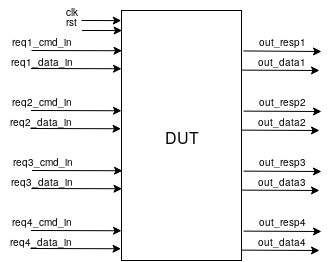
\includegraphics[width=80mm]{img/v5_dut.png}
  \caption{DUT}
  \label{fig:dut}
\end{figure}

U narednoj tabeli je opisan interfejs našeg DUT-a.\\

\begin{table}[h!]
  \centering
  \rowcolors{1}{white!15}{gray!30}
  \begin{tabular}{|l|l|l|l|}
    \hline
    \textbf{Ime} & \textbf{Širina (br. bita)} & \textbf{Smer} & \textbf{Opis}\\
    \hline
    c\(\_\)clk & 1 & in & takt\\
    \hline
    reset & 8 & in & reset\\
    \hline
    reg1\(\_\)cmd\(\_\)in & 4 & in & komanda za port 1\\
    \hline
    reg1\(\_\)data\(\_\)in & 32 & in & podaci za port 1\\
    \hline
    reg2\(\_\)cmd\(\_\)in & 4 & in & komanda za port 2\\
    \hline
    reg2\(\_\)data\(\_\)in & 32 & in & podaci za port 2\\
    \hline
    reg3\(\_\)cmd\(\_\)in & 4 & in & komanda za port 3\\
    \hline
    reg3\(\_\)data\(\_\)in & 32 & in & podaci za port 3\\
    \hline
    reg4\(\_\)cmd\(\_\)in & 4 & in & komanda za port 4\\
    \hline
    reg4\(\_\)data\(\_\)in & 32 & in & podaci za port 4\\
    \hline
    out\(\_\)resp1 & 2 & out & odgovor za port 1\\
    \hline
    out\(\_\)data1 & 32 & out & rezultat za port 1\\
    \hline
    out\(\_\)resp2 & 2 & out & odgovor za port 2\\
    \hline
    out\(\_\)data2 & 32 & out & rezultat za port 2\\
    \hline
    out\(\_\)resp3 & 2 & out & odgovor za port 3\\
    \hline
    out\(\_\)data3 & 32 & out & rezultat za port 3\\
    \hline
    out\(\_\)resp4 & 2 & out & odgovor za port 4\\
    \hline
    out\(\_\)data4 & 32 & out & rezultat za port 4\\
    \hline
  \end{tabular}
  \caption{DUT interfejs}
  \label{tab:dut_if}
\end{table}

Kao što se vidi u tabeli \ref{tab:dut_if}, svaki od četiri porta ima po dva
ulazna i dva izlazna signala. \emph{regX\(\_\)cmd\(\_\)in} signal je
četvorobitni ulazni signal za slanje komande. U tabeli \ref{tab:dut_commands} su
prikazane moguće komande i njihova vrednost.\\

\begin{table}[h!]
  \centering
  \rowcolors{1}{white!15}{gray!30}
  \begin{tabular}{|l|l|}
    \hline
    \textbf{Komanda} & \textbf{Vrednost}\\
    \hline
    \emph{No operation} & 4\textquotesingle b0000\\
    \hline
    \emph{Add} & 4\textquotesingle b0001\\
    \hline
    \emph{Subtract} & 4\textquotesingle b0010\\
    \hline
    \emph{Shift left} & 4\textquotesingle b0101\\
    \hline
    \emph{Shift right} & 4\textquotesingle b0110\\
    \hline
    \emph{Invalid} & sve preostale vrednosti\\
    \hline
  \end{tabular}
  \caption{DUT komande}
  \label{tab:dut_commands}
\end{table}

\emph{regX\(\_\)data\(\_\)in} je 32-bitni ulaz za podatke. Dva podatka koji
predstavljaju operande se šalju na ovoj liniji, pri čemu se prvo šalje operand
1, a zatim operand 2 u sledećem taktu. Operand 1 se šalje u istom taktu kada i
komanda. I odavde vidimo da je potrebno dva takta da bi se poslao zahtev DUT-u.
U zavisnosti od komande, ova dva operanda se tumače na različite načine, koji su
prikazani u tabeli \ref{tab:dut_operands}.\\

\begin{table}[h!]
  \centering
  \rowcolors{1}{white!15}{gray!30}
  \begin{tabular}{|l|p{0.8\textwidth}|}
    \hline
    \textbf{Komanda} & \textbf{Tumačenje operanada}\\
    \hline
    \emph{Add} & Rezultat je operand1 + operand2\\
    \hline
    \emph{Subtract} & Rezultat je operand1 - operand2\\
    \hline
    \emph{Shift left} & Rezultat je operand1 šiftovan u levo za operand2 mesta, pri čemu se koriste samo 5 bita drugog operanda. Uvek se ubacuju nule.\\
    \hline
    \emph{Shift right} & Rezultat je operand1 šiftovan u desno za operand2 mesta, pri čemu se koriste samo 5 bita drugog operanda. Uvek se ubacuju nule.\\
    \hline
  \end{tabular}
  \caption{DUT operandi}
  \label{tab:dut_operands}
\end{table}

Postoje i dve izlazne linije za svaki port. \emph{out\(\_\)respX} je dvobitni
signal za odgovor koji daje informacije o uspešnosti operacije. Vrednosti su:\\

\begin{table}[h!]
  \centering
  \rowcolors{1}{white!15}{gray!30}
  \begin{tabular}{|l|p{8cm}|}
    \hline
    \textbf{Vrednost} & \textbf{Značenje}\\
    \hline
    2\textquotesingle b00 & Nema odgovora u ovom ciklusu.\\
    \hline
    2\textquotesingle b01 & Uspešna operacija. Rezultujući podaci se nalaze na \emph{out\(\_\)dataX} liniji.\\
    \hline
    2\textquotesingle b10 & \emph{Overflow}, \emph{underflow} ili pogrešna komanda. \emph{Overflow/underflow} je moguć samo za operacije sabiranja i oduzimanja.\\
    \hline
    2\textquotesingle b11 & Ne koristi se.\\
    \hline
  \end{tabular}
  \caption{DUT odgovor}
  \label{tab:dut_response}
\end{table}

Rezultat operacije se nalazi na \emph{out\(\_\)dataX} liniji i validan je jedino
u ciklusima u kojima je \emph{out\(\_\)respX} = 2\textquotesingle b01, odnosno kada je operacija
uspešna.\\

Na slici \ref{fig:calc_port1} je prikazana uspešna operacija na portu 1. Komanda
i prvi operand se šalju u jednom ciklusu, a drugi operand se šalje u narednom
ciklusu. Nakon nekoliko taktova dobija se odgovor i rezultat u istom ciklusu.
Broj ciklusa koji je potreban da se dobije odgovor zavisi od aktivnosti na
ostalim portovima (pošto postoje samo dve ALU), ali će uvek biti minimum 3
ciklusa.\\

\begin{figure}[h!]
  \centering
  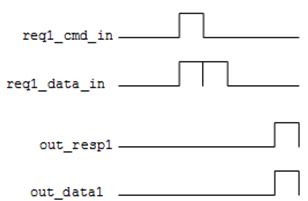
\includegraphics[width=60mm, scale=0.5]{img/v5_p1.png}
  \caption{Primer operacije na portu 1}
  \label{fig:calc_port1}
\end{figure}

Na svakom portu može biti aktivna samo jedna operacija, odnosno kada se pošalje
jedna komanda, sledeća se ne sme slati do god ne primimo odgovor za prvu
komandu. Takođe, slanje nove komande je opciono tj. port može biti neaktivan.\\

Četiri porta su nezavisna. Mogu se paralelno slati komande na svim ili samo
nekim portovima, što znači da u bilo kom trenutku DUT može obavljati maksimum 4
operacije. Međutim, brzina odgovora će zavisiti od aktivnosti zbog ograničenih
resursa u dizajnu. Kako što je već rečeno, DUT sadrži dve ALU, jednu za
sabiranje i oduzimanje, a drugu za šiftovanje. Ukoliko se primi više komandi u
paraleli za jednu ALU, DUT će ih serijalizovati i obrađivati jednu po jednu.
Svaki port ima isti prioritet. DUT će obrađivati komande po principu
\emph{first-come, first-serve}, pri čemu za komande koje stignu u istom taktu
nije definisan redosled.\\

Što se tiče reseta, aktiviranje se vrši postavljanjem reset linije na vrednost
8\textquotesingle b11111111. Ova vrednost se mora držati 7 sukcesivnih taktova kako bi se reset
uspešno propagirao kroz dizajn. Tokom reseta, svi ulazi, osim takta, treba da
budu nula.\\

U ``Calc1'' dizajnu se sve aritmetičke operacije vrše nad \emph{unsigned}
podacima. Prilikom sabiranja \emph{overflow} se dešava ukoliko najviši bit ima
\emph{carry-out}. Slično \emph{underflow} se pojavljuje prilikom oduzimanja
ukoliko se oduzima veći broj od manjeg broja. U nastavku je dato par primera.\\

\begin{table}[h!]
  \centering
  \rowcolors{1}{white!15}{gray!30}
  \begin{tabular}{|l|l|l|l|l|}
    \hline
    \textbf{Komanda} & \textbf{Operand 1} & \textbf{Operand 2} & \textbf{Odgovor} & \textbf{Rezultat}\\
    \hline
    \emph{Add} & 32\textquotesingle h80002345 & 32\textquotesingle h00010000 & Uspešna operacija & 32\textquotesingle h80012345\\
    \hline
    \emph{Add} & 32\textquotesingle hFFFFFFFF & 32\textquotesingle h00000001 & \emph{Overflow} & Nema\\
    \hline
    \emph{Subtract} & 32\textquotesingle hFFFFFFFF & 32\textquotesingle h11111111 & Uspešna operacija & 32\textquotesingle hEEEEEEEE\\
    \hline
    \emph{Subtract} & 32\textquotesingle h11111111 & 32\textquotesingle h20000000 & \emph{Underflow} & Nema\\
    \hline
  \end{tabular}
  \caption{DUT primeri operacija}
  \label{tab:dut_examples}
\end{table}

%========================================================================================
% Section
%========================================================================================

\section{\emph{Data (sequence) item}}

Kao što je već navedeno, na ovim vežbama ćemo izvršiti verifikaciju ``Calc1''
dizajna. Prilikom razvoja verifikacionih okruženja, jedan od prvih koraka je
implementacija klase koja predstavlja transakciju. U literaturi se sreću mnogi
termini za ovaj objekat uključujući \emph{data item, sequence item, frame,
  packet, transaction}, ...\\

\emph{Data (sequence) item} predstavlja transakciju koja se koristi kao
stimulus. Koristi se na mnogim mestima u verifikacionom okruženju uključujuci
slanje podataka od sekvencera ka drajveru. Slanjem više ovih transakcija ka
drajveru se kreiraju sekvence koje su osnova za generisanje stimulusa. Veza
između drajvera i sekvencera, kao i način pisanja sekvenci će biti detaljno
opisani u narednoj vežbi, dok je u ovoj vežbi fokus na modelovanju transakcija.
Sama transakcija treba da sadrži sve informacije potrebne drajveru da ispravno
generiše signale na interfejsu, ali može i sadržati neke dodatne podatke koji
služe za kontrolu.\\

Ove transakcije će se implementirati kao klase koje nasleđuju (direktno ili
indirektno) \emph{uvm\(\_\)sequence\(\_\)item} klasu. Polja u klasi zavise od
potreba drajvera, nivoa apstrakcije, ali i potreba ostatka okruženja. Uglavnom
se ti podaci mogu podeliti u nekoliko grupa:

\begin{itemize}
\item Kontrolna polja - npr. tip transfera, veličina, ...
\item \emph{Payload} polja - sami podaci koji se šalju, npr. vrednost adrese
\item Konfiguraciona polja - npr. ponašanje prilikom grešaka
\item Polja za analizu - pomoćna polja koja olakšavaju analizu, npr. vreme
\end{itemize}

Sam princip generisanja stimulusa u \emph{constrained-random} verifikaciji se
zasniva na randomizaciji ovih transackija kako bi se pokrili interesantni
scenariji. Samim tim, veliki broj polja je često deklarisan kao \emph{rand}, uz
određena ograničenja kako bi se generisale željene transakcije.\\

Sadržaj transakcija je opisan na primeru transakcije za APB i UART protokol.
U ovom primeru se vidi da transackija može sadržati željeni broj polja, ali i
metode koje olakšavaju njeno korišćenje (u primeru UART \emph{seq item}-a
postoji metoda za računanje parnosti).\\

\lstinputlisting[caption=Primer APB transakcije, label=lst:apb_seq_item]{code/v5_apb_seq_item.sv}

\lstinputlisting[caption=Primer UART transakcije, label=lst:uart_seq_item]{code/v5_uart_seq_item.sv}

Nasleđivanjem iz \emph{uvm\(\_\)sequence\(\_\)item} klase i korišćenjem raznih
UVM field makroa, omogućava se korišćenje mnogobrojnih metoda za rad sa ovom
klasom uključujući \emph{print, copy, compare} itd.
Primer ispisa print metode je takođe dat ispod.
Vidi se da korišćenje ovih metoda može biti veoma korisno i umnogome olakšati \emph{debug}.\\

\begin{verbatim}
# ------------------------------------------------
# Name          Type        Size   Value
# ------------------------------------------------
# uart_frame    uart_frame  -      @366
#  start_bit    integral    1      'h0
#  payload      integral    8      'hcc
#  parity       integral    1      'h1
#  stop_bits    integral    2      'h3
#  error_bit    integral    4      'h0
#  parity_type  parity_e    1      GOOD_PARITY
#  delay        integral    32     'd13
# ------------------------------------------------
\end{verbatim}

%========================================================================================
% Section
%========================================================================================

\section{Simulacija}

% ----------------------------------------------------------------------------------------

\subsection{Kompilacija}

Prilikom kompajliranja koda koji sadrži UVM biblioteku, potrebno je uključiti
direktorijum koji sadrži UVM kod. Npr. (ukoliko UVM\(\_\)HOME pokazuje na sors
kod):

\begin{lstlisting}
vlog -sv +incdir+$env(UVM_HOME) calc_verif_top.sv
\end{lstlisting}
% $

Napomena: ova podešavanja se odnose na alat koji se koristi na vežbama.
Kod novijih verzija alata podešavanja mogu biti drugačija.

% ----------------------------------------------------------------------------------------

\subsection{UVM \emph{command line processor}}

\emph{Command line processor} klasa pruža mogućnosti preuzimanja informacija
koje se daju preko komandne linije prilikom poziva simulacije. Mogućnosti ovog
procesora su mnogobrojne i izlaze iz opsega ovog kursa. Mi ćemo se zadržati na
podešavanjima samo nekoliko UVM varijabli sa komandne linije koje umnogome
olakšavaju simulaciju - podešavanje opširnosti ispisa poruka (\emph{verbosity})
i definisanje testa koji se pušta. Za detaljnije objašnjenje rada
\emph{uvm\(\_\)cmdline\(\_\)processor} klase pogledati ``UVM Users Guide'',
poglavlje 6.6.\\

Test se pušta pozivom \emph{run\(\_\)test(\textless test\(\_\)name\textgreater
  )} rutine u top modulu. Tada se kreira instanca datog testa i pokreće se
simulacija. Sledeći primer pokreće test pod nazivom \emph{test\(\_\)example}:

\begin{lstlisting}
module top;

  import uvm_pkg::*;
  `include "uvm_macros.svh"

  // instantiate the DUT, connect,
  initial begin
    run_test("test_example");
  end
endmodule : top
\end{lstlisting}

Mane ovakvog pristupa su očigledne - svaki put kada želimo da pustimo drugi
test, mora se menjati sors kod. Zbog toga se u praksi uvek koristi komandna
linija za izbor testa. Kada se \emph{run\(\_\)test} pozove bez argumenta,
proverava se +UVM\(\_\)TESTNAME=\textless test\(\_\)name\textgreater\ opcija.
Sada se ne mora menjati sors kod, odnosno može se puštati više testova bez
ponovnog kompajliranja čime se znatno štedi na vremenu. Primer prosleđivanja
testa preko komandne linije:

\begin{lstlisting}
vsim top +UVM_TESTNAME=test_example
\end{lstlisting}

+UVM\(\_\)VERBOSITY opcija pruža mogućnost promene verbosity u čitavom okruženju
odnosno kontrolu ispisa poruka. Nivoi su opisani u drugom poglavlju ove vežbe
(UVM\(\_\)LOW, UVM\(\_\)HIGH, ...). Primer upotrebe:

\begin{lstlisting}
vsim top +UVM_VERBOSITY=UVM_HIGH
\end{lstlisting}

+UVM\(\_\)MAX\(\_\)QUIT\(\_\)COUNT opcija pruža mogućnost završetka simulacije
kada se dostigne dati broj grešaka u dizajnu. Ova opcija je posebno korisna
tokom puštanja regresije. Podrazumevana vrednost je -1 odnosno simulacija se
nikad ne završava na osnovu broja grešaka. Pod brojem grešaka se podrazumeva
broj prijavljenih \emph{uvm\(\_\)error}-a.

%========================================================================================
% Section
%========================================================================================

\section{Zadaci}

\paragraph{Zadatak}

U pratećim fajlovima za ovu vežbu je povezan naš DUT sa interfejsom i kreiran
kostur za UVM test klasu. Proučiti date fajlove i način puštanja testova.
Za dati DUT kreirati \emph{sequence item} klasu koja će sadržati potrebna
polja. Na osnovu funkcionalne specifikacije zaključiti koja polja treba da
sadrži ova klasa. Da li će polja biti \emph{rand} i zašto? Napisati ograničenja
za randomizaciju ukoliko su potrebna.

\paragraph{Zadatak}

Napisati test koji instancira \emph{sequence item} kreiran u prethodnom zadatku,
randomizuje ga i u \emph{main} fazi ispisuje vrednost svih polja.
Pokrenuti test i preko komandne linije kontrolisati ispis poruka.

%========================================================================================
% Section
%========================================================================================

\section{Appendix}

\lstinputlisting[caption=calc\(\_\)if, label=lst:calc_if]{code/calc_if.sv}
\lstinputlisting[caption=v5\(\_\)calc\(\_\)verif\(\_\)pkg, label=lst:v5_calc_verif_pkg]{code/v5_calc_verif_pkg.sv}
\lstinputlisting[caption=v5\(\_\)calc\(\_\)verif\(\_\)top, label=lst:v5_calc_verif_top]{code/v5_calc_verif_top.sv}
\lstinputlisting[caption=v5\(\_\)test\(\_\)simple, label=lst:v5_test_simple]{code/tests/v5_test_simple.sv}
\lstinputlisting[language=tcl, caption=calc\(\_\)run, label=lst:calc_run]{code/calc_run.do}

%========================================================================================
